\tocless\subsubsection{Concurrent Separation Logic}

In order to reason about heap manipulating programs, separation logic was introduced in \cite{seplogic} as a program logic which revolves around the concept of resource owning. The program state does not just involve values local to a method, but also ones that live in the shared \textit{heap} and that variables refer to through pointers. In terms of assertions, the main additions to Hoare's constructs are explained in the following list.
\begin{itemize}
\item The separating conjunction $P \lstar Q$ asserts that the state can be divided into two disjoint parts, one of which satisfies predicate $P$ and the other one $Q$.
\item $\cell{E_1}{E_2}$ asserts that there exists a memory cell whose address can be obtained by evaluating $E_1$ and whose value is $E_2$.
\item The empty assertion $emp$ states that the \textit{heap} must contain no allocated cells.
\end{itemize}

The separating conjunction empowers the program logic to have a frame rule which allows to prove a specification by temporarily not considering additional resources in the heap that are not accessed as part of the command we are verifying.

\[
	\infer
	{\vdash \triple{P \lstar R}{C}{Q \lstar R}}
	{\vdash \triple{P}{C}{Q} \ \ \pred{mod}{C} \cap \pred{fv}{R} \equiv \emptyset}
\]

The requirement for it to work, is that no variable which is modified as part of running command $C$ can be free in predicate $R$. Another way of looking at the rule is that if we are able to prove a triple, then adding an arbitrary resource, which is not touched by the command, will not invalidate our original proof. In later work, O'Hearn \cite{csl} included support for disjoint concurrency through a new rule.
\begin{gather*}
	\infer
	{\vdash \triple{P_1 \lstar P_2}{C_1\ ||\ C_2}{Q_1 \lstar Q_2}}
	{
		\vdash \triple{P_1}{C_1}{Q_1} &
		\vdash \triple{P_2}{C_2}{Q_2} &
		\pred{nc}{C_1, C_2, P_2, Q_2} &
		\pred{nc}{C_2, C_1, P_1, Q_1}
	}
	\\[0.8em]
	\pred{nc}{C, C', P, Q} \triangleq \pred{mod}{C} \cap (\pred{fv}{C'} \cup \pred{fv}{P} \cup \pred{fv}{Q}) \equiv \emptyset
\end{gather*}

The rule states that as long as two threads only access disjoint parts of memory to execute, then they can safely be composed in parallel. The disjointness requirement appears as a side-condition to the rule, expressed through the non conflict predicate $\mathsf{nc}$.

When dealing with process interaction, programs need to be syntactically structured in a new way. This novelty is introduced in order to declare and model the shared resources which are accessible to concurrent commands in a program. On top this, a new command is also introduced to allow a process to access shared resources through a conditional critical region \cite{csl} \cite{brookes}.
\[
	\begin{array}{c | c}
		\begin{array}{l}
			init; \\
			\texttt{resource } r_1(\text{vars}), \ldots r_m(\text{vars}) \\
			C_1 \| \cdots \| C_n
		\end{array}
		&
		\begin{array}{l}
			C ::= \cdots\ |\ \texttt{with } r \texttt{ when } B \texttt{ do } C \texttt{ endwith}
		\end{array}
	\end{array}
\]
Shared resources are uniquely named and have a list of input variables that they manage. A process can interact with them using the ``\texttt{with}" command, representing a unit of mutual exclusion. Access is only granted if no other region on $r$ is currently executing and the boolean condition $B$ (which is heap independent) evaluates to true. In all other cases the process must wait for the described conditions to become true.

Each declared resource $r_i$ is assigned a resource invariant in the shape of a formula $RI_{r_i}$. The latter needs to be precise and any assignment $\passign{x}{\cdots}$, where $x$ is a free variable in $RI_{r_i}$, must occur within a conditional critical region for $r_i$. The proof rules are enhanced to be able to cover the new syntactic constructs. First, all of the resource invariants must be separately established by the initialization list of commands $init$, together with a part of the state, i.e. $P'$, that can be accessed outside of critical regions. The latter is the only assertion used to prove that $Q$ holds on conclusion of the parallel execution of commands $C_1 \| \cdots \| C_n$. All of the invariants are then established again as part of the rule's conclusion.
\[
	\infer
	{
		\vdash \triple
		{P}
		{
			\begin{array}{l}
				init; \\
				\texttt{resource } r_1(\text{vars}), \ldots r_m(\text{vars}) \\
				C_1 \| \cdots \| C_n
			\end{array}
		}
		{RI_{r_1} \sep \cdots \sep RI_{r_m} \sep Q}
	}
	{
		\vdash \triple
		{P}
		{init}
		{RI_{r_1} \sep \cdots \sep RI_{r_m} \sep P'} &
		\vdash \triple
		{P'}
		{C_1 \| \cdots \| C_n}
		{Q}
	}
\]

Whenever a conditional critical region command for $r$ is encountered, and no other process is within a region for the same resource, we add the resource invariant $RI_{r_i}$ to the process' local state. Using this approach, when a process is outside a region for $r$, it is effectively not able to see $r$'s state.
\[
	\begin{array}{c c}
		\begin{array}{c}
		\infer
		{
			\vdash \triple
			{P}
			{\texttt{with } r \texttt{ when } B \texttt{ do } C \texttt{ endwith}}
			{Q}
		}
		{
			\vdash \triple
			{(P \sep RI_r) \land B}
			{C}
			{Q \sep RI_r}
		}
		\end{array}
		&
		\begin{array}{l}
			\text{No other process modifies} \\
			\text{variables free in $P$ or $Q$}
		\end{array}
	\end{array}
\]

It follows that the parallel composition rule does not change from the disjoint case, given that any shared resource invariant is absent from $P_1, \ldots, P_n$ and $Q_1, \ldots, Q_n$ and will only be added at the appropriate moment, within a critical region.
\[
	\infer
	{
		\vdash \triple
		{P_1 \sep \cdots \sep P_n}
		{C_1 \| \cdots \| C_n}
		{Q_1 \sep \cdots \sep Q_n}
	}
	{
		\vdash \triple
		{P_1}{C_1}{Q_1} &
		\cdots &
		\vdash \triple
		{P_n}{C_n}{Q_n}
	}
\]


\tocless\subsubsection{RGSep} \label{rgsep}

The efforts developed as part of separation logic and rely/guarantee reasoning were brought together by RGSep \cite{viktor}. Its main contribution was related to the separation between the local state $l$ and shared one $s$. In an abstract sense, $l$ and $s$ are members of a separation algebra $(M, \odot, \mathsf{u})$ such that $l \odot s$ is defined if and only if the two are disjoint \cite{sepalgebra}. In the latter case, the entirety of the state is defined to be the union of $l$ and $s$. In order to distinguish them, a new kind of assertion, the shared assertion, is introduced and often referred to as the ``boxed assertion". In fact, $\boxed{P}$ expresses a generic separation logic assertion $P$ which refers to the shared state $s$. The separating conjunction $\lstar$ works in the usual way inside of the local state but behaves additively for the shared one. As a consequence we have that $\boxed{P} \lstar \boxed{Q} \Leftrightarrow \boxed{P \land Q}$.

Interference between parallel threads is modelled using actions of the form $P \transto Q$. The action meaning is that the part of the shared state where $P$ holds will be replaced with a part that satisfies $Q$ leaving the rest of $s$ intact. For example, if we were describing the action that allows to increment a counter stored at address $x$, we would have something along the lines of $\cell{x}{n} \transto \cell{x, m} \land m \geq n$.

RGSep requires all preconditions and postconditions of commands in a proof to be stable under interference coming from the environment. We can syntactically check for stability as follows.
\begin{align*}
\pred{stable}{S, \sem{P \transto Q}} &\Leftrightarrow\ \vDash ((P \sepimp S) \lstar Q) \Rightarrow S
\\
\pred{stable}{S, (R_1 \cup R_2)^*} &\Leftrightarrow\ \vDash \pred{stable}{S, R_1} \land \pred{stable}{S, R_2}
\end{align*}
The first property states that if we take a state $S$ and remove the part satisfying $P$ and add one where $Q$ holds then $S$ will hold again. On the other hand, the second property defines that a statement is stable with respect to a set of actions when it is stable under the interference of every action in the set. Given that actions can only affect the shared state $s$, the stability check only needs to be performed on assertions which refer to $s$ itself. \\

\tocless\subsubsection{Concurrent Abstract Predicates}

\label{sec:cap}

Concurrent Abstract Predicates (CAP) is a program logic explained in \cite{cap} which makes use of separation logic constructs to allow abstraction on shared data structures using abstract predicates. These provide a disjointness of shared resources at the abstraction level which might not be reflected in the actual implementation. For example, if we consider a set module and formulate a predicate stating that ``the set is $\{ 1,2 \}$", then we want to remove element $2$ and be able to assert that the set is now $\{ 1 \}$. In order to reason about the module in such a fine-grained manner, we want element $2$ to be manipulated independently from the rest of the set. This kind of disjointness expressed at the level of abstraction does not need to be part of the implementation. In fact one could implement the set module using a singly linked list which requires traversing some elements before reaching the desired item.

Concurrent abstract predicates also hold information regarding what kind of interference is allowed on the shared memory from the thread and the environment. Fractional permissions are utilized in order to model the type of control a thread has on a particular shared structure \cite{fractional}. On top of this, implementation code can be formally verified against high level specifications and later be \textit{hidden} to clients that make use of it by allowing them not to refer to low-level details in their own proof derivations.

Standard separation logic is augmented with two novel assertions, the shared region and the permission one. The first takes the shape $\sharedr{P}$ and represents a part of memory, associated with an identifier $r$, which is shared among several threads and satisfies predicate $P$. The region is indivisible so that all threads accessing it always get a consistent view of it; we can enforce such behaviour as follows:
\[
	\sharedr{P} \lstar \sharedr{Q} \iff \sharedr{P \land Q}
\]

The permission assertion $[\tguard{A}]_\pi^r$ gives the thread the possibility to perform action $\tguard{A}$ on region $r$ with fractional permission $\pi$. The latter will be a real value in $(0, 1)$ when both the thread and the environment can execute $\tguard{A}$ or equals to $1$ in the case where the thread is the only one to be able to do so. We can combine permissions to perform the same action in the same region in the following way:
\[
	[\tguard{A}]_{\pi_1}^r \lstar [\tguard{A}]_{\pi_2}^r \iff [\tguard{A}]_{\pi_1 + \pi_2}^r
\]

Actions in CAP are similar to the ones seen in Section \ref{rgsep} and have the form $\tguard{A}: P \transto Q$ where the label is followed by two assertions that describe the part of the region needed for $\tguard{A}$ and the same part after the action has taken place. All possible actions for a particular region $r$ are summarized inside $I(r, \vec{x})$. We can create a shared region from an assertion $P$ as $P \Rrightarrow \exists r \ldotp \sharedr{P} \lstar \pred{all}{I(r, \vec{x})}$, by including every action permission available.

We now have all the ingredients to prove the specification \cite{cap} of a lock module in CAP. The latter will provide three methods, namely \texttt{makeLock()}, \texttt{lock(x)} and \texttt{unlock(x)}. As the names suggest, the first method will allocate the necessary resources for a lock and initiate it while the other two will acquire or release the lock at address $\pvar{x}$. Following these English specifications we can provide formal ones.
\begin{gather*}
\triple
{emp}
{\mathtt{makeLock}()}
{\exists x \ldotp \pvar{ret} = x \land \pred{isLock}{x} \lstar \pred{Locked}{x}}
\\
\triple
{\pred{isLock}{\pvar{x}}}
{\mathtt{lock}(\pvar{x})}
{\pred{isLock}{\pvar{x}} \lstar \pred{Locked}{\pvar{x}}}
\\
\triple
{\pred{Locked}{\pvar{x}}}
{\mathtt{unlock}(\pvar{x})}
{emp}
\end{gather*}

The actions allowed on the lock are $\tguard{L}$ and $\tguard{U}$ which are used to interpret the abstract predicates used in the specification.
\begin{align*}
\pred{isLock}{x} &\equiv \exists r, \pi \ldotp [\tguard{L}]_\pi^r \lstar \sharedrs{(\cell{x}{0} \lstar [\tguard{U}]_1^r) \lor \cell{x}{1}}
\\
\pred{Locked}{x} &\equiv \exists r \ldotp [\tguard{U}]_1^r \lstar \sharedrs{\cell{x}{1}}
\\
I(r, x) &\triangleq 
\left\lbrace
\begin{array}{rl}
\tguard{L}: & [\tguard{U}]_1^r \lstar \cell{x}{0} \transto \cell{x}{1} \\
\tguard{U}: & \cell{x}{1} \transto [\tguard{U}]_1^r \lstar \cell{x}{0}
\end{array}
\right\rbrace
\end{align*}

The $\pred{isLock}{x}$ predicate gives a thread knowledge of the existence of a lock at address $x$ which can either be in the locked or unlocked state based on the value $x$ points to. It also provides a permission to perform the $\tguard{L}$ action to acquire the lock. Given the nature of the predicate we can state that $\pred{isLock}{x} \Rightarrow \pred{isLock}{x} \lstar \pred{isLock}{x}$ holds as we are simply sharing the knowledge of $x$ being a lock.

\begin{figure}[h]
\[
\begin{array}{@{}l@{\qquad}l@{\qquad}l@{}}
	\begin{array}{@{}l@{}}
	\pfunctions{makeLock}{} \\
		\quad \palloc{\pvar{x}}{1}; \\
		\quad \pmutate{\pvar{x}}{1}; \\
		\quad \preturn{\pvar{x}}; \\
	\pfunctione
	\end{array}
	&
	\begin{array}{@{}l@{}}
	\pfunctions{lock}{\pvar{x}} \\
		\quad \mathtt{do}\ \{ \\
			\quad \quad \patomic{\pfuncall{\pvar{b}}{CAS}{\pvar{x}, 0, 1}}; \\
		\quad \}\ \mathtt{while}\ (\pvar{b} = 0); \\
	\pfunctione
	\end{array}
	&
	\begin{array}{@{}l@{}}
	\pfunctions{unlock}{\pvar{x}} \\
		\quad \patomic{\pmutate{\pvar{x}}{0}}; \\
	\pfunctione
	\end{array}
\end{array}
\]
\captionof{figure}{A spin lock implementation using \texttt{CAS}.}
\label{fig:spinlock}
\end{figure}

On the other hand, $\pred{Locked}{x}$ describes that the lock at $x$ is currently locked and has been previously acquired by the thread that holds the predicate. As the $\pred{Locked}{x}$ predicate gives us full permission of $[\tguard{U}]_1^r$, we have that $\pred{Locked}{x} \lstar \pred{Locked}{x} \Rightarrow \bot$ since a thread cannot acquire the lock twice sequentially. Action $\tguard{L}$'s effect requires the lock to be unlocked and for the region to include the permission to perform $\tguard{U}$. In fact, once the action is performed, the latter permission will be removed from the region and included in the thread's local state so that no other thread can release the lock. $\tguard{U}$ has instead the opposite behaviour: it requires the lock to be acquired and once done, it will put the unlock permission back in the shared region. The specification provided will be used to verify a concrete implementation of the lock module using a spin lock whose code is given in Figure \ref{fig:spinlock}.

The \texttt{lock} method uses a popular mechanism to handle synchronization, namely compare-and-swap. \texttt{CAS}($a$, $c$, $v$) works by atomically comparing the dereferenced value of $a$ with $c$ and in case of a match, $a$ is set to point to $v$. In case of a successful swap, \texttt{CAS} returns 1, otherwise it returns 0.

\begin{figure}[h]
\[
\begin{array}{l}
\specline{\pred{isLock}{\pvar{x}}} \\
\pfunctions{lock}{\pvar{x}} \\
	\quad \specline{\exists r, \pi \ldotp [\tguard{L}]_\pi^r \lstar \sharedrs{(\cell{\pvar{x}}{0} \lstar [\tguard{U}]_1^r) \lor \cell{\pvar{x}}{1}}} \\
	\quad \mathtt{do}\ \{ \\
		\quad \quad \patomic{\pfuncall{\pvar{b}}{CAS}{\pvar{x}, 0, 1}}; \\
		\quad \quad \specline{\exists r, \pi \ldotp \left( [\tguard{L}]_\pi^r \lstar \sharedrs{(\cell{\pvar{x}}{0} \lstar [\tguard{U}]_1^r) \lor \cell{\pvar{x}}{1}} \land \pvar{b} = 0 \right) \\ \lor \left( [\tguard{L}]_\pi^r \lstar [\tguard{U}]_1^r \lstar \sharedr{\cell{\pvar{x}}{1}} \land \pvar{b} = 1 \right)} \\
	\quad \}\ \mathtt{while}\ (\pvar{b} = 0); \\
	\quad \specline{[\tguard{L}]_\pi^r \lstar [\tguard{U}]_1^r \lstar \sharedr{\cell{\pvar{x}}{1}}} \\
\pfunctione \\
\specline{\pred{isLock}{\pvar{x}} \lstar \pred{Locked}{\pvar{x}}}
\end{array}
\]
\captionof{figure}{The spin lock's \texttt{lock} function implementation proof.}
\label{fig:spinproof}
\end{figure}

In Figure \ref{fig:spinproof} we give a CAP sketch proof of the \texttt{lock(x)} method which is shown to satisfy its specification. Note how the use of \texttt{CAS} is combined with a while loop whose condition is the outcome of the swap. This way we can be sure that once the control flow of the program exits the loop, the lock's state is updated and the $\tguard{L}$ action has taken place.

\tocless\subsubsection{Abstract atomicity and Linearizability}

We refer to an operation as atomic when it happens at a single discrete point in time \cite{modularsteps}. Whenever atomic actions are performed concurrently, the actual execution will always be an interleaving of those. In general, even if a command is built from multiple operations, abstract atomicity can be obtained if the overall effect appears to be atomic.

Linearizability \cite{linearizability} is a correctness condition which allows methods of a concurrent module to be used by clients as atomic. All of such module operations are provided with sequential specifications that are proven to behave atomically with respect to each other. As a consequence, the moment a new method is added to the module, the linearizability proof for all methods needs to be performed. The main contribution of the approach is the fact that specifications that guarantee linearizability are an abstraction which can be directly used by clients of the module to reason without having to worry about the implementation details. \\

\tocless\subsubsection{TaDA} \label{s:tada}

TaDA \cite{tada} is a modern program logic that combines the perks of the CAP approach and of linearizability to allow modular proofs of concurrent programs. Its main novelty is the introduction of atomic specifications as a first-order construct through the use of atomic triples. These have the form $\atriplenl{}{x \in X}{P(x)}{C}{Q(x)}$ and indicate that command $C$ will atomically update the state from $P$ to $Q$ in a single, discrete step.

\begin{center}
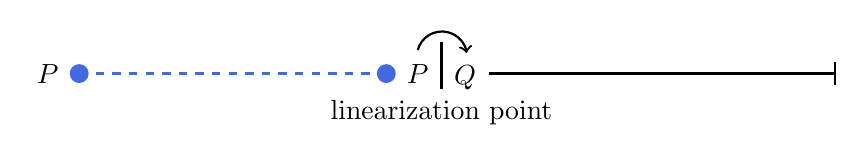
\begin{tikzpicture}[thick]
\node (Ps) at (0, 0) {$P$};
\node (P) at (4.7, 0) {$P$};
\node (Q) at (5.3, -0.05) {$Q$};
\node (L) at (5, -0.5) {linearization point};

\filldraw[color=RoyalBlue] (0.4, 0) circle (3pt);
\filldraw[color=RoyalBlue] (4.3, 0) circle (3pt);
\draw[color=RoyalBlue, dashed] (0.4, 0) -- (4.3, 0);
\draw (5, 0.4) -- (5, -0.2);
\draw (5.6, 0) -- (10, 0);
\draw (10, 0.15) -- (10, -0.15);
\draw [->] (4.7, 0.3) arc (165:8:9pt); 
\end{tikzpicture}
\end{center}

More specifically, the triple actually states that, due to the environment's interference, the variable bound by the pseudo-quantifier $\aall$ (in this case $x$) can vary within the values of set $X$ as long as it still satisfies precondition $P(x)$. Then, right at the function's linearization point, the $C$ command will atomically bring the state to satisfy $Q(x)$. After this, the command does not give any guarantees on the validity of $Q(x)$ since it might be changed by another thread running concurrently. On the other hand, $C$ will not change the state of $x$ again after the linearization point but it can use it to refer to its value right before the event. The specifications give a notion of atomicity which is only maintained at the level of abstraction defined by $P$. In fact, observing the state at a lower level might show several distinct steps involved as part of the command.

We will explore TaDA's rules and constructs while going through a concrete program example of a stack data structure module, which supports concurrent access. The concurrent stack module will have a simple interface for clients to use that allows the creation of a new stack and the ability to push and pop items from it.

Note that the full atomic triple has the following shape, where the first part of the state is private to the thread:
\[
	\atriplee{}{x \in X}{P_p}{P(x)}{C}{y \in Y}{Q_p(x, y)}{Q(x, y)}
\]
This includes all assertions which are stable under the environment's intereference. Everything which is instead on the public side of the state, accepts interference as described by the guarded transitions for regions. Whenever we encounter a standard Hoare triple $\triple{P}{C}{Q}$ in TaDA, we can see it as pure syntactic sugar for $\atriplenq{}{P}{\top}{C}{Q}{\top}$ where there is effectively no public state.	
\begin{gather*}
\triple{emp}{\mathtt{makeStack}()}{\exists r \ldotp \pred{S}{r, \pvar{ret}, []}}
\\[0.7em]
\atriplenl
{}
{l}
{\pred{S}{r, \pvar{x}, l} \land \pvar{v} \neq 0}
{\pfuncallnr{push}{\pvar{x}, \pvar{v}}}
{\pred{S}{r, \pvar{x}, \pvar{v}\cons l}}
\\[0.7em]
\vatriplenl
{}
{l}
{\pred{S}{r, \pvar{x}, l}}
{\mathtt{pop}(\pvar{x})}
{(\pred{S}{r, \pvar{x}, []} \land \pvar{ret} = 0) \lor (\exists l'\ldotp \pred{S}{r, \pvar{x}, l'} \land l = \pvar{ret}\cons l' \land \pvar{ret} \neq 0)}
\end{gather*}

The \texttt{makeStack()} method is given a sequential specification, since it would be unreal to use a shared structure during its creation. In a more likely setup, a single thread creates the stack and then passes its reference to other (potentially child) threads. The function's return value will be a pointer to the new data structure. Adding elements to the stack is done through the use of \texttt{push}(\texttt{x},\texttt{v}) which puts the item \texttt{v} on top of the stack. We require an atomic specification for the method as the environment might interact with the structure while we are pushing to it. The inserted value must be different from $0$ due to the fact that the return value of \texttt{pop(x)} will be $0$ in the case of an empty stack. This is just a simplified convention, given the abscence of error handling in this demonstrating example. The abstract predicate $\pred{S}{r, x, l}$, in a style similar to CAP, indicates the presence of a stack in the shared region identified by $r$, at memory address $x$ with contents $l$. We can formally define it as follows.
\begin{align*}
\pred{S}{r, x, l} &\triangleq \exists h, ns, ds \ldotp \textbf{Stack}_r(x, h, ns, ds) \lstar [\tguard{G}]_r \land l = \pred{values}{ns}
\\
\text{where } &\pred{values}{[]} \triangleq []
\\
&\pred{values}{(-, v) \cons l} \triangleq v \cons \pred{values}{l}
\end{align*}

The region type $\textbf{Stack}_r(x, h, ns, ds)$ described the structure of a shared region in memory. In addition to that, $[\tguard{G}]_r$ is a guard that is associated to the region as an abstract resource. It gives a thread the permission to perform action $\tguard{G}$ on shared region $r$. Actions in TaDA are defined inside a labelled transition system that maps guards to possible updates to the region. In our case, we express a single guard which gives the ability to both push and pop from the stack. In the second case, the update actually only happens when the stack is non-empty.
\begin{align*}
&\tguard{G}: \forall n, v \neq 0, ns, ds \ldotp (ns, ds) \transto ((n, v) \cons ns, ds)
\\
&\tguard{G}: \forall n, v, ns, ds \ldotp (ns, ds) \transto \ite{ns = (n, v) \cons ns'}{(ns', (n, v) \cons ds)}{(ns, ds)}
\end{align*}

We unveil the meaning of the additional arguments of $\textbf{Stack}_r$ by providing a region interpretation for the latter.
\begin{align*}
I(\textbf{Stack}_r(x, h, ns, ds)) \triangleq &\cell{x}{h} \lstar \mathsf{stack}(h, ns) \lstar \bigoast_{(n, v) \in ds} \twocell{n}{v}{-}
\\
\text{where } &\mathsf{stack}(h, []) \triangleq h = \snull
\\
&\mathsf{stack}(h, (h, v) \cons l) \triangleq v \neq 0 \land \exists z . \twocell{h}{v}{z} \lstar \mathsf{stack}(z, l)
\end{align*}

The stack's address $x$ points to the head node, $h$, which is the first node of the structure that will be either $\snull$ for an empty stack or point to a value and a subsequent node. On top of this, $ns$ is a logical list including all active node pairs $(n, v)$ in the stack where $n$ is the node's address and $v$ the value it points to. Those nodes that were at one point part of the stack but have been popped since, are called dead nodes and included in the set $ds$. As we can see from the transition system, every time an item is popped, it is virtually moved from $ns$ to $ds$ to keep track of it. This additional information, which can be seen as a ghost state of the program, is particularly helpful when proving the \texttt{pop} function implementation. In fact, if the function pops an item $n$ which has been concurrently removed since we first read it, then it is necessary to know that it had the $\twocell{n}{-}{-}$ structure and this information is provided as part of the dead nodes assertion.

\begin{figure}[h]
\[
	\begin{array}{l}
		\pfunction{\pvar{makeStack}}
		{}
		{
		\\
		\quad \palloc{\pvar{x}}{1};
		\\
		\quad \preturn{\pvar{x}}; \\
		}
		\end{array}
		\ \ \ \
		\begin{array}{l}
		\pfunction{\pvar{push}}
		{\pvar{x}, \pvar{v}}
		{
		\\
		\quad \palloc{\pvar{fst}}{2};
		\\
		\quad \pmutate{\pvar{fst}}{\pvar{v}};
		\\
		\\
		\quad \mathtt{do} \ \{
		\\
		\quad \quad \pderef{\pvar{h}}{\pvar{x}};
		\\
		\quad \quad \pmutate{\pvar{fst} + 1}{\pvar{h}};
		\\
		\quad \quad \pfuncall{\pvar{b}}{CAS}{\pvar{x}, \pvar{h}, \pvar{fst}};
		\\
		\quad\} \ \mathtt{while}\ (\pvar{b} = 0);
		\\
		}
		\end{array}
		\ \ \ \
		\begin{array}{l}
		\pfunction{\pvar{pop}}
		{\pvar{x}}
		{
		\\
		\quad \passign{\pvar{r}}{0};
		\\
		\quad \mathtt{do} \ \{
		\\
		\quad \quad \passign{\pvar{b}}{0};
		\\
		\quad \quad \pderef{\pvar{h}}{\pvar{x}};
		\\
		\quad\quad \pifelses{\pvar{h} = \snull}
		\\
		\quad\quad \quad \preturn{0};
		\\
		\quad\quad \pifelsem
		\\
		\quad \quad \quad \pderef{\pvar{r}}{\pvar{h}};
		\\
		\quad \quad \quad \pderef{\pvar{next}}{\pvar{h} + 1};
		\\
		\quad \quad \quad \pfuncall{\pvar{b}}{CAS}{\pvar{x}, \pvar{h}, \pvar{next}};
		\\
		\quad\quad \pifelsee
		\\
		\quad\} \ \mathtt{while}\ (\pvar{b} = 0);
		\\
		\\
		\quad \preturn{\pvar{r}};
		\\
		}
	\end{array}
	\label{fig:concurrentstack}
	\]
	\captionof{figure}{The concurrent stack \textsc{While} language implementation with the addition of the compare-and-swap (\texttt{CAS}) command.}
\end{figure}

We provide an implementation of the three methods in Figure \ref{fig:concurrentstack} followed by a full TaDA proof of the $\pfuncallnr{push}{\pvar{x}, \pvar{v}}$ function in Figure \ref{fig:tadaProof}. The proof begins by unwrapping the $\pred{S}{r, \pvar{x}, l}$ abstract predicate into its definition which includes the $\textbf{Stack}_r$ region predicate and the $[\tguard{G}]_r$  action guard. We use the latter as part of the \textsc{MakeAtomic} rule, in order to modify the underlying stack structure to insert a new element, $\pvar{v}$. This step gives us the atomicity tracking component $\atomtok$ and the ability of treating a sequence of commands as if they happened atomically. As part of the function's body, we allocate memory for the node (\texttt{fst}) that will host the new element and begin a loop whose task is to read the stack's head node into \texttt{h} and use \texttt{CAS} to atomically set it to \texttt{fst} only when \texttt{h} is equivalent to $[\pvar{x}]$ (meaning that the value of the stack's head has not changed since we first read it into \texttt{h}). We prove all of this using the following inference rules:
\begin{itemize}
\item \textsc{Existential} in order to get rid of the existential quantifiers on logical variables $h, ns, ds$ and to be able to apply the next rules.
\item The \textsc{AWeakening} rule to turn the logical variables $h, ns, ds$ into pseudo-quantified ones (bound by $\aall$) and to prove an atomic triple referring to the update that follows.
\item \textsc{UpdateRegion} consumes the atomicity tracking component to try and update the shared region $\textbf{Stack}_r$ by first opening it up and revealing its interpretation. Later, the update can either succeed or fail, as described by the rule's postcondition that includes a disjunction.
\item We \textsc{Frame} out all assertions only leaving $\cell{\pvar{x}}{h}$ since this is all we need to conclude the proof. In fact, the $\pfuncallnr{CAS}{\pvar{x}, \pvar{h}, \pvar{fst}}$ command does not modify any other variables a part from $\pvar{x}$.
\item The \textsc{CAS} rule finally allows us to condition the actual update on the boolean return value, $\pvar{b}$ which is used inside the following postconditions to understand whether the swap has happened or not.
\end{itemize}

\newgeometry{margin=2cm}
\begin{center}
\[
\small{
\begin{array}{@{\hspace*{-20pt}}l}
	\quantifierline{\aall l \ldotp} \\
	\aspecline{\pred{S}{r, \pvar{x}, l} \land \pvar{v} \neq 0} \\
	\pfunction{\pvar{push}}{\pvar{x}, \pvar{v}}{ \\
		\quad \aspecline{\pred{S}{r, \pvar{x}, l} \land \pvar{v} \neq 0} \\
		\quad \begin{leftvruled}{abstract}
			\aspecline{\exists h, ns, ds \ldotp \textbf{Stack}_r(\pvar{x}, h, ns, ds) \lstar [\tguard{G}]_r \land l = \pred{values}{ns} \land \pvar{v} \neq 0} \\
			\begin{leftvruled}{atomic exists on $ns$, $ds$}
				\quantifierline{\aall ns, ds \ldotp} \\
				\aspecline{\exists h \ldotp \textbf{Stack}_r(\pvar{x}, h, ns, ds) \lstar [\tguard{G}]_r \land l = \pred{values}{ns} \land \pvar{v} \neq 0} \\
				\begin{leftvruled}{make atomic}
					\acontextline{r : (ns, ds) \transto ((-, \pvar{v}) \cons ns, ds) \land \pvar{v} \neq 0 \vdash} \\
					\specline{\exists h, ns, ds \ldotp \textbf{Stack}_r(\pvar{x}, h, ns, ds) \land l = \pred{values}{ns} \lstar r \Mapsto \atomtok \land \pvar{v} \neq 0} \\
					\palloc{\pvar{fst}}{2}; \pmutate{\pvar{fst}}{\pvar{l}}; \\
					\specline{\exists h, ns, ds \ldotp \textbf{Stack}_r(\pvar{x}, h, ns, ds) \land l = \pred{values}{ns} \lstar r \Mapsto \atomtok \lstar \twocell{\pvar{fst}}{\pvar{v}}{\snull} \land \pvar{v} \neq 0} \\
					\mathtt{do} \ \{ \\
						\quad \specline{\exists h, ns, ds, s \ldotp \textbf{Stack}_r(\pvar{x}, h, ns, ds) \land l = \pred{values}{ns} \lstar r \Mapsto \atomtok \lstar \twocell{\pvar{fst}}{\pvar{v}}{s} \land \pvar{v} \neq 0} \\
						\quad \begin{leftvruled}{open region}
							\quantifierline{\aall h, ns, ds \ldotp}
							\aspecline{\cell{\pvar{x}}{h} \lstar \mathsf{stack}(h, ns) \lstar \bigoast_{(n, v) \in ds} \twocell{n}{v}{-}} \\
							\begin{leftvruled}{frame}
								\quantifierline{\aall h \ldotp} \aspecline{\cell{\pvar{x}}{h}} \\
								\pderef{\pvar{h}}{\pvar{x}}; \\
								\aspecline{\cell{\pvar{x}}{h} \land \pvar{h} = h}
							\quad \end{leftvruled} \\
							\aspecline{\cell{\pvar{x}}{h} \lstar \mathsf{stack}(h, ns) \lstar \bigoast_{(n, v) \in ds} \twocell{n}{v}{-} \land \pvar{h} = h} \\
						\end{leftvruled} \\
						\quad \specline{\exists h, ns, ds, s, a \ldotp \textbf{Stack}_r(\pvar{x}, h, ns, ds) \land l = \pred{values}{ns} \lstar r \Mapsto \atomtok \lstar \twocell{\pvar{fst}}{\pvar{v}}{s} \land \pvar{h} = a \land \pvar{v} \neq 0} \\
						\quad \pmutate{\pvar{fst} + 1}{\pvar{h}}; \\
						\quad \specline{\exists h, ns, ds \ldotp \textbf{Stack}_r(\pvar{x}, h, ns, ds) \land l = \pred{values}{ns} \lstar r \Mapsto \atomtok \lstar \twocell{\pvar{fst}}{\pvar{v}}{\pvar{h}} \land \pvar{v} \neq 0} \\
						\quad \begin{leftvruled}{existential on $h, ns, ds$}
							\specline{\textbf{Stack}_r(\pvar{x}, h, ns, ds) \land l = \pred{values}{ns} \lstar r \Mapsto \atomtok \lstar \twocell{\pvar{fst}}{\pvar{v}}{\pvar{h}} \land \pvar{v} \neq 0} \\
							\begin{leftvruled}{weakening on $h$, $ns$, $ds$}
								\quantifierline{\aall h, ns, ds \ldotp} \\
								\aspecline{\textbf{Stack}_r(\pvar{x}, h, ns, ds) \land l = \pred{values}{ns} \lstar r \Mapsto \atomtok \lstar \twocell{\pvar{fst}}{\pvar{v}}{\pvar{h}} \land \pvar{v} \neq 0} \\
								\begin{leftvruled}{update region}
									\aspecline{\cell{\pvar{x}}{h} \lstar \mathsf{stack}(h, ns) \lstar \bigoast_{(n, v) \in ds} \twocell{n}{v}{-} \land l = \pred{values}{ns} \lstar \twocell{\pvar{fst}}{\pvar{v}}{\pvar{h}} \land \pvar{v} \neq 0} \\
									\begin{leftvruled}{frame, CAS}
										\quantifierline{\aall h \ldotp} \\
										\aspecline{\cell{\pvar{x}}{h}} \\
										\pfuncall{\pvar{b}}{CAS}{\pvar{x}, \pvar{h}, \pvar{fst}}; \\
										\aspecline{(\pvar{b} = 0 \land \cell{\pvar{x}}{h} \land \pvar{h} \neq h)
										\lor (\pvar{b} = 1 \land \cell{\pvar{x}}{\pvar{fst}} \land \pvar{h} = h)}
									\end{leftvruled} \\
									\aspecline{(\pvar{b} = 0 \land \pvar{h} \neq h \land \cell{\pvar{x}}{h} \lstar
									\mathsf{stack}(h, ns) \lstar \twocell{\pvar{fst}}{\pvar{v}}{\pvar{h}}) \\
									\lor (\pvar{b} = 1 \land \pvar{h} = h \land \cell{\pvar{x}}{\pvar{fst}} \lstar
									\twocell{\pvar{fst}}{\pvar{v}}{\pvar{h}} \lstar \mathsf{stack}(\pvar{h}, ns)) \\
									\lstar \bigoast_{(n, v) \in ds} \twocell{n}{v}{-} \land l = \pred{values}{ns} \land \pvar{v} \neq 0}
								\end{leftvruled} \\
								\aspecline{l = \pred{values}{ns} \land \pvar{v} \neq 0 \land ((\pvar{b} = 0 \land \textbf{Stack}_r(\pvar{x}, h, ns, ds) \lstar \twocell{\pvar{fst}}{\pvar{v}}{\pvar{h}} \lstar r \Mapsto \atomtok) \\
								\lor (\pvar{b} = 1 \land \textbf{Stack}_r(\pvar{x}, h, (\pvar{fst}, \pvar{v}) \cons ns, ds)) \lstar r \Mapsto ((ns, ds), ((-, \pvar{v}) \cons ns, ds)))}
							\end{leftvruled} \\
							\specline{((\pvar{b} = 0 \land \textbf{Stack}_r(\pvar{x}, h, ns, ds) \lstar \twocell{\pvar{fst}}{\pvar{v}}{\pvar{h}} \lstar r \Mapsto \atomtok) \\ \lor (\pvar{b} = 1 \lstar r \Mapsto ((ns, ds), ((-, \pvar{v}) \cons ns, ds))) \land l = \pred{values}{ns} \land \pvar{v} \neq 0}
						\end{leftvruled} \\
						\quad \specline{\exists h, ns, ds \ldotp ((\pvar{b} = 0 \land
						\textbf{Stack}_r(\pvar{x}, h, ns, ds) \lstar \twocell{\pvar{fst}}{\pvar{v}}{\pvar{h}}
						\lstar r \Mapsto \atomtok) \\
						\lor (\pvar{b} = 1 \lstar r \Mapsto ((ns, ds), ((-, \pvar{v}) \cons ns, ds)))  \land l = \pred{values}{ns} \land \pvar{v} \neq 0} \\
					\} \ \mathtt{while}(\pvar{b} = 0); \\
					\specline{\exists h, ns, ds \ldotp l = \pred{values}{ns} \lstar r \Mapsto ((ns, ds), ((-, \pvar{v}) \cons ns, ds))} \\
				\end{leftvruled} \\
				\aspecline{\exists h \ldotp \textbf{Stack}_r(\pvar{x}, h, (-, \pvar{v}) \cons ns, ds) \lstar [\tguard{G}]_r \land l = \pred{values}{ns}} \\
			\end{leftvruled} \\
			\aspecline{\exists h, ns, ds \ldotp \textbf{Stack}_r(\pvar{x}, h, (-, \pvar{v}) \cons ns, ds) \lstar [\tguard{G}]_r \land l = \pred{values}{ns}} \\
		\end{leftvruled} \\
		\quad \aspecline{\pred{S}{r, \pvar{x}, \pvar{v}\cons l}} \\
	}
\end{array}
}
\]
\captionof{figure}{Sketch TaDA proof of the \texttt{push} concurrent stack method.}
\label{fig:tadaProof}
\end{center}
\restoregeometry

As part of the logic, there are some key inference rules that are displayed in the \texttt{push} proof. For an exhaustive list and explanation we point the reader to \cite{tada}. First of all, \textsc{MakeAtomic} allows to take an atomic specification and prove the abstract atomicity of a sequence of non-atomic commands where a single linearization point will appear and update the shared state. In order to do so, we must hold the guard of the appropriate action for the region. In the premiss, we obtain the atomicity tracker component in the form of an abstract resource ($\atomtok$). This works like a token used to recognize whether the atomic update declared in the atomicity context ($\acontextline{a : x \transto f(x)}$) has already happened or not. On a successful update, the token will be converted into the state transition described by the guarded action. As we can see from the postcondition of the premiss, the atomic update \textit{must} happen at some point in order to satisfy the rule.
\begin{gather*}
f : X \rightarrow Y \ \ \left\lbrace (x, y)\ |\ x \in X, y \in f(x) \right\rbrace \subseteq \mathcal{T}_\textbf{t}^* \\
\infer
{
\atriplenl
	{}
	{x \in X}
	{\textbf{t}_a(\vec{z}, x) \lstar [\tguard{G}]_a}
	{C}
	{\exists y \in f(x) \ldotp \textbf{t}_a(\vec{z}, y) \lstar [\tguard{G}]_a}
}
{
\triplena
	{\acontextline{a : x \in X \transto f(x)}}
	{\exists x \in X \ldotp \textbf{t}_a(\vec{z}, x) \lstar a \Mapsto \atomtok}
	{C}
	{\exists x \in X, y \in f(x) \ldotp a \Mapsto (x, y)}
}
\\
\textsc{MakeAtomic}
\end{gather*}

The moment we need to access the contents of a shared region to unveil its interpretation, we can use one of two rules: \textsc{OpenRegion} and \textsc{UpdateRegion}. The first one allows to view the underlying content of a region but it forbids any update to its abstract state. For this reason, it neither needs an explicit guard nor a tracking component to be used. On the other hand the \textsc{UpdateRegion} rule is employed to perform the atomic update of the region's abstract state. It requires the update not to have happened already and we can guarantee that with the presence of the atomicity token in the precondition. Inside the postcondition we need to take into account whether the update has succeeded or not and we do that by having a disjunction on the two possible predicates that hold for the region.
\begin{gather*}
\infer
{
\atriplenl
{\acontextline{a : x \in X \transto f(x)}}
{x \in X}
{\textbf{t}_a(\vec{z}, x) \lstar P(x) \\
	\lstar a \Mapsto \atomtok}
{C}
{\exists y \in f(x) \ldotp \textbf{t}_a(\vec{z}, y) \\ \lstar Q_1(x, y) \lstar
		a \Mapsto (x, y) \lor \\ \textbf{t}_a(\vec{z}, x) \lstar Q_2(x) \lstar a \Mapsto \atomtok}
}
{
\atriplenl
	{}
	{x \in X}
	{I(\textbf{t}_a(\vec{z}, x)) \lstar P(x)}
	{C}
	{\exists y \in f(x) \ldotp I(\textbf{t}_a(\vec{z}, y)) \lstar Q_1(x, y) \\
		\lor I(\textbf{t}_a(\vec{z}, x)) \lstar Q_2(x)}
}
\\
\textsc{UpdateRegion}
\end{gather*}

Another way to update a shared region is to apply the \textsc{UseAtomic} rule which grants the permission to perform such change through an explicit guard held in the precondition, in contrast with the atomicity tracking component in \textsc{UpdateRegion}. The use of this inference rule implies that command $C$ acts atomically at an abstraction level which is lower than the one of region $a$ and as a consequence, it will be atomic at the higher level as well. This way we can stack a layer of abstraction on top of another which gives a lot of flexibility in terms of writing program modules that extend or make use of other pre-verified modules.
\begin{gather*}
f : X \rightarrow Y \ \ \left\lbrace (x, y)\ |\ x \in X, y \in f(x) \right\rbrace \subseteq \mathcal{T}_\textbf{t}^* \\
\infer
{
\atriplenl
{}
{x \in X}
{\textbf{t}_a(\vec{z}, x) \lstar [\tguard{G}]_a}
{C}
{\exists y \in f(x) \ldotp \textbf{t}_a(\vec{z}, y) \lstar [\tguard{G}]_a}
}
{
\atriplenl
{}
{x \in X}
{I(\textbf{t}_a(\vec{z}, x)) \lstar [\tguard{G}]_a}
{C}
{\exists y \in f(x) \ldotp I(\textbf{t}_a(\vec{z}, y)) \lstar [\tguard{G}]_a}
}
\\
\textsc{UseAtomic}
\end{gather*}

Finally, the \textsc{Frame} rule works in the same way as in separation logic, by adding resources to the precondition and postcondition of a command that does not modify them. As we can notice in the \texttt{push} proof, we can also frame out predicates referring to variables bound by $\aall$.
\begin{gather*}
\pred{mod}{C} \cap \pred{vars}{R_p} \equiv \emptyset\ \
\pred{mod}{C} \cap \pred{vars}{R(x)} \equiv \emptyset \\
\infer
{
	\atriple
	{}
	{x \in X}
	{P_p \lstar R_p}
	{P(x) \lstar R(x)}
	{C}
	{Q_p(x, y) \lstar R_p}
	{Q(x, y) \lstar R(x)}
}
{
	\atriplee
	{}
	{x \in X}
	{P_p}
	{P(x)}
	{C}
	{y \in Y}
	{Q_p(x, y)}
	{Q(x, y)}
}
\\
\textsc{Frame}
\end{gather*}